
\documentclass{article}
\usepackage{../../../LaTeX-Preamables/Assign}
\usepackage{amsmath} % Required for \text{} in math mode if needed

\begin{document}
\newcommand{\documentcourse}{IIMT2641}
\newcommand{\documentnumber}{5} % Updated assignment number

% ------------------------------------ %
%                Header                %
% ------------------------------------ %

\begin{minipage}{0.07\textwidth}
    
\includegraphics[width=\linewidth]{../../../LaTeX-Preamables/LaTeX-Templates/HKULOGO256.png}
\end{minipage}
\hspace{0.02\textwidth}
\begin{minipage}{0.55\textwidth}
    \documentcourse

    Assignment \documentnumber

    SID: 3036268218
\end{minipage}
\begin{minipage}{0.35\textwidth}
    \begin{flushright}
        Jax

        \jobname.pdf

        \today
    \end{flushright}
\end{minipage}

\vspace{0.5cm}

\hrule

% ------------------------------------ %
%                Content               %
% ------------------------------------ %

\begin{enumerate}[label=\alph*.]
      \item Hierarchical Clustering
            \begin{enumerate}[label=(\roman*)]
                  \item Building hierarchical clustering model takes two steps. For the first step, we have to calculate the distances between each point. This process will have to process $n$ elements for each $n$ elements. For the second step, we have to merge the closest points or clusters, described by the following algorithm:
                        \begin{enumerate}
                              \item Start with each data point in the cluster including itself only
                              \item Compute the distance between each pair of clusters
                              \item Combine the two nearest clusters
                              \item Re-compute the distance between each pair of clusters
                              \item Combine the two nearest clusters
                              \item Repeat 4 and 5 until all data points belong to one single cluster
                        \end{enumerate}
                        As we have over 3k observations and 1.5k variables, the process will be lengthy and time-consuming.

                  \item Dendrogram:

                        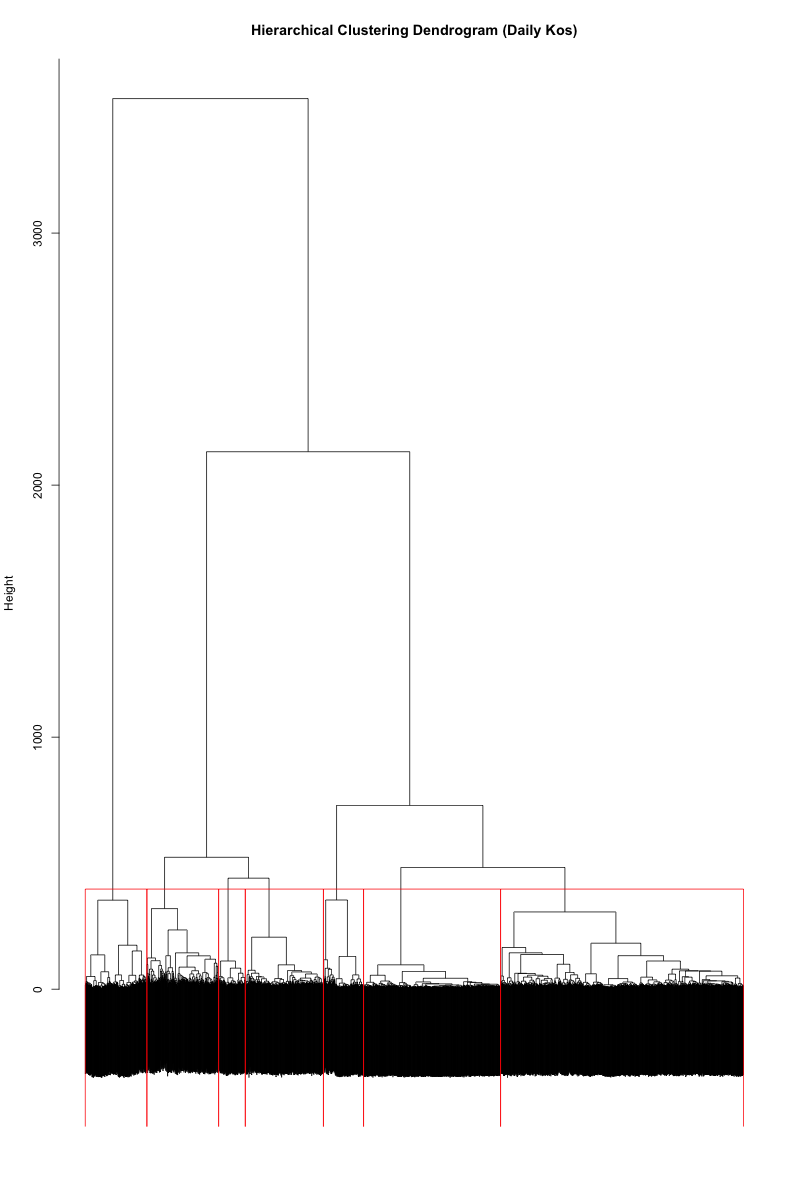
\includegraphics[width=.5\textwidth]{./5/plot.png}

                        I picked the number of clusters to be $7$, as this gives a good balance of \textit{wiggle room} and number of topics a reader would potentially be interested in and want to read about.

                  \item The number of observations in each of the 7 hierarchical clusters are:
                        \begin{enumerate}[label=\arabic*/]
                              \item 1266 observations
                              \item 321 observations
                              \item 374 observations
                              \item 139 observations
                              \item 407 observations
                              \item 714 observations
                              \item 209 observations
                        \end{enumerate}

                  \item The top 6 words for each hierarchical cluster are:
                        \begin{enumerate}[label=\arabic*/]
                              \item \texttt{state, republican, poll, democrat, kerry, bush}

                                    State level politics and polls
                              \item \texttt{bush, democrat, challenge, vote, poll, november}

                                    Challenges of the november election
                              \item \texttt{elect, parties, state, republican, democrat, bush}

                                    State level elections and parties
                              \item \texttt{campaign, voter, presided, poll, bush, kerry}

                                    Campaign process
                              \item \texttt{american, presided, administration, war, iraq, bush}

                                    Mostly about \textbf{[Iraq war]}
                              \item \texttt{race, bush, kerry, elect, democrat, poll}

                                    Electoral races
                              \item \texttt{democrat, clark, edward, poll, kerry, dean}

                                    Mostly about \textbf{[Democratic party]}
                        \end{enumerate}
            \end{enumerate}

      \item K-means Clustering (using $k=7$)
            \textbf{K-means Clustering Analysis:}
            \begin{enumerate}[label=(\roman*)]
                  \item \textbf{Cluster Sizes:} The number of observations in each K-means cluster are as follows:
                        \begin{enumerate}[label=\arabic*/]
                              \item 515 observations
                              \item 159 observations
                              \item 1880 observations
                              \item 270 observations
                              \item 326 observations
                              \item 147 observations
                              \item 133 observations
                        \end{enumerate}
                        The cluster sizes are different because we used different fundamentally algorithms for generating clusters.

                  \item \textbf{Cluster Word Analysis:} The top 6 most frequent words for each K-means cluster are, and matching with the hierarchical clusters:
                        \begin{enumerate}[label=\arabic*/]
                              \item general, campaign, presided, poll, kerry, bush $\to$ 4
                              \item race, senate, state, parties, republican, democrat $\to$ 6
                              \item kerry, elect, republican, poll, democrat, bush $\to$ 3
                              \item iraqi, american, administration, war, bush, iraq $\to$ 5
                              \item bush, democrat, challenge, vote, poll, november $\to$ 2
                              \item primaries, democrat, edward, clark, kerry, dean $\to$ 7
                              \item percent, democrat, presided, poll, kerry, bush $\to$ 1
                        \end{enumerate}
                        Although the key words don't match completly, the key themes can be matched to each identified clusters from the heirarchical clustering.

            \end{enumerate}

\end{enumerate}
\end{document}
